%!TeX spellcheck = en_GB
% ****** Start of file templateForReport.tex ******

% TeX'ing this file requires that you have all prerequisites
% for REVTeX 4.1 installed
%
% See the REVTeX 4 README file
% It also requires running BibTeX. The commands are as follows:
%
%  1)  latex templateForReport.tex
%  2)  bibtex templateForReport
%  3)  latex templateForReport.tex
%  4)  latex templateForReport.tex
%
\documentclass[%
 reprint,
%superscriptaddress,
%groupedaddress,
%unsortedaddress,
%runinaddress,
%frontmatterverbose,
%preprint,
%showpacs,preprintnumbers,
%nofootinbib,
%nobibnotes,
%bibnotes,
 amsmath,amssymb,
 aps,
%pra,
%prb,
%rmp,
%prstab,
%prstper,
%floatfix,
]{revtex4-1}

\usepackage{graphicx}% Include figure files
\usepackage{dcolumn}% Align table columns on decimal point
\usepackage{bm}% bold math
%\usepackage{hyperref}% add hypertext capabilities
%\usepackage[mathlines]{lineno}% Enable numbering of text and display math
%\linenumbers\relax % Commence numbering lines

%\usepackage[showframe,%Uncomment any one of the following lines to test
%%scale=0.7, marginratio={1:1, 2:3}, ignoreall,% default settings
%%text={7in,10in},centering,
%%margin=1.5in,
%%total={6.5in,8.75in}, top=1.2in, left=0.9in, includefoot,
%%height=10in,a5paper,hmargin={3cm,0.8in},
%]{geometry}

\usepackage{dsfont} % mathds for unity matrix
\usepackage{bbold} % mathbb for unity matrix
\usepackage{physics}% integral measure
\usepackage{xcolor}
\usepackage{tikz}%Bilder
\usepackage{pgfpages}
\usetikzlibrary{positioning, arrows}
\usepackage{smartdiagram}%Kreisdiagramm/Flussdiagramm
\usepackage{siunitx}   % Intelligentes Setzen von Zahlen und Einheiten

%\DeclareMathOperator{\Tr}{Tr}
\renewcommand{\Re}{\operatorname{Re}}

\begin{document}
	\tikzstyle{arrow} = [very thick, ->, >=stealth]

\title{Yang-Mills on the Lattice}% Force line breaks with \\
%\thanks{A footnote to the article title}%

\author{Nico Dichter}
\author{Christiane Gro\ss{}}


\date{March 2021}% It is always \today, today,
             %  but any date may be explicitly specified

\begin{abstract}
	We measure the confinement that arises when simulating a lattice with the Yang-Mills action, by approximating the lattice links with SU(N) matrices. It is known that the confinement arises from using non abelian gauge fields. The confinement is characterized by the linear rise of the potential between two quarks.
%  An article usually includes an abstract, a concise summary of the work
%  covered at length in the main body of the article.
%  \begin{description}
%  \item[Usage]
%    Secondary publications and information retrieval purposes.
%  \item[Structure]
%    You may use the \texttt{description} environment to structure your abstract;
%    use the optional argument of the \verb+\item+ command to give the category of each item.
%  \end{description}
\end{abstract}
\maketitle

%\tableofcontents

\section{Introduction}

Quarks as fundamental particles have been postulated since the 1960s, however no free quarks have ever been observed, only colourless bound quark states have been observed. QCD attempts to describe this confinement, but no analytical proof of this description has been given. Analytically solving this would be one of the steps to solving the connected millenium problem of the Yang-Mills spectrum. Numerically, confinement has been shown, and this report aims to reproduce these findings for the easiest case of static quarks, which do not change location.
This corresponds to infinitely heavy quarks. More background is given by e.\,g.\, \citet{lepagelqcd} and \citet{povhparticles}.

We discretize the spacetime as a lattice, and use observables calculated with this lattice to extract the potential for various distances.

%
%What are we doing? Extracting the potential between static quarks interacting under Yang-Mills theory. 
%Why is that important? The potential shows us whether to expect confinement, explaining why free quarks are not/cannot be observed.
%Why SU(n)? SU(3) simulates the strong interaction, however SU(2) is easier and faster to calculate.
%Why are we interested in this lattice/this action? Basis for the spectra of glueballs, a millenium problem.

%We want to calculate the potential between two infinitely heavy quarks. To do this, we first simulate an empty lattice and then use the fact that static quarks do not vary their location when the time is varied.

\section{Theoretical basis}

Most of the theoretical basis given here is adapted from \citet{lepagelqcd}. We want to discretise three spatial and one temporal dimension, so we need a four-dimensional lattice. The distance between any adjacent lattice points is $a$, and any point is characterized by four coordinates, $x=(x,y,z,t)$. The links between the lattice sites are characterized by an additional direction $\hat{\mu}$, and we only consider the forward facing links $U_\mu(x)$ going from $x$ to $x+a\hat{\mu}$. All links are represented as $SU(N)$-matrices, we simulate $N=2$ and $N=3$. Backward-facing links from $x+a\hat{\mu}$ to $x$ are represented by $U_\mu^\dagger(x)$.

The simplest loop that can be formed with the links of the lattice is the plaquette \[P_{\mu\nu}(x)=\frac{1}{N}\Re\tr\left(U_\mu(x)U_\nu(x+a\hat{\mu})U_\mu^\dagger(x+a\hat{\nu})U^\dagger_\nu(x)\right)\] a simple square. These link variables $U_\mu$ are connected to the continuum in the following way: The Yang Mills action in the continuum reads as \[S=\int\dd{^4x}\dfrac{1}{2}\sum\limits_{\mu,\nu}\tr F_{\mu\nu}²(x)\] where the field tensor\[F_{\mu\nu}=\partial_\mu A_\nu-\partial_\nu A_\mu+\i g [A_\mu,A_\nu]\] is a traceless N$\times$N hermitian matrix with $g$ the coupling strength. The standard discretization connects the gauge fields $A_\mu$ to the link variables $U_\mu$, \[U_\mu(x)=\mathcal{P}\exp(-\i\int\limits_{x}^{x+a\hat{\mu}}g A\cdot\dd{y})\]
Here the $\mathcal{P}$-Operator orders the integrand along the path from $x$ to $x+a\hat{\mu}$.

The discretized version of the Yang Mills action is defined as being proportional to the ordered sum over all plaquettes, \[S=\frac{2N}{g^2}\sum_{x}\sum_{\mu>\nu}\left(1-P_{\mu\nu}(x)\right)+\mathcal{O}(a^2)\]
and $\beta:=\frac{2N}{g^2}$. We are interested in observables of the form $\langle O\rangle=\frac{1}{Z}\int \dd \vec{o} O(\vec{o}) \exp(-\beta S(\vec{o}))$, with $ Z=\int \dd \vec{o} O(\vec{o}) \exp(-\beta S(\vec{o}))$ and $\vec{o}$ a possible lattice configuration. Generating our ensembles so they are $\sim \frac{1}{Z} \exp(-\beta S(\vec{o}))$ allows the expectation value to be calculated as a simple mean.

\citet{creutzsu2} says the expectation value for the plaquette for SU(2) goes like $\langle P \rangle=\beta/4$ for strong coupling, i.\,e.\, $\beta\to 0$ and like $\langle P \rangle =1-\frac{3}{4\beta}$ for weak coupling, i.\,e.\, $\beta\to \infty$.

%Some citation \citet{gsldoc_complex}

%Most of the theoretical basis given here is adapted from \citet{lepagelqcd}. We simulate a lattice with one temporal and three spatial dimensions, with the distande $a$ between neighbouring points. The nearest neighbours in this lattice are linked, with the links characterized by SU(2) or SU(3) matrices $U_\mu(x)$, where $\mu=0\dots3$ is the direction of the link. Backwards links are defined as the hermitian adjoint of the forward-facing link. The plaquette is the smallest possible square on the lattice and is defined as $P_{\mu\nu}(x)=\frac{1}{N}\Re\Tr\left(U_\mu(x)U_\nu(x+a\mu)U_\mu^\dagger(x+a\nu)U^\dagger_\nu(x)\right)$, where $N$ describes the dimension of the unitary matrices used to simulate the links. Building on this, we define the action to be $S=\frac{2N}{g^2}\sum_{x}\sum_{\mu>\nu}\left(1-P_{\mu\nu}(x)\right)$.
%
%Definition wilson-loop: maybe draw loop? How?
%

%\[W(x, k_\mu a, l_\nu a)=U_\mu(x)\cdots U_\mu(x+(k-1)a\mu)U_\nu(x+ka\mu)\cdots U_\nu(x+ka\mu+(l-1)a\nu)U_mu^dagger\]

A general loop around a closed contour $\mathcal{C}$ is also called Wilson loop $W(\mathcal{C})$. Regarding the more complicated loops possible, we are interested in $W(R,  T)$ that go a distance $R$ in the spatial directions and a distance $T$ in the temporal direction. Their expectation values can be calculated as 

\begin{tikzpicture}[y=0.5cm, x=0.5cm,
roundnode/.style={circle, draw=white, thick, minimum size=1pt},
]
\node[roundnode]at(-4.0, 1)(equation){$W(R, T)=\frac{1}{N}\Re\tr$};
\node[roundnode]at(2.5, -0.8)(R){R};
\draw[arrow] (2,-0.8)--(0,-0.8);
\draw[arrow] (3,-0.8)--(5,-0.8);
\node[roundnode]at(5.8, 1)(T){T};
\draw[arrow] (5.8, 1.5)--(5.8,2);
\draw[arrow] (5.8, 0.5)--(5.8,0);
\filldraw[black] (0,0) circle (2pt);
\draw[arrow] (0,0)--(1,0);
\filldraw[black] (1,0) circle (2pt);
\draw[arrow] (1,0)--(2,0);
\filldraw[black] (2,0) circle (2pt);
\draw[arrow] (2,0)--(3,0);
\filldraw[black] (3,0) circle (2pt);
\draw[arrow] (3,0)--(4,0);
\filldraw[black] (4,0) circle (2pt);
\draw[arrow] (4,0)--(5,0);
\filldraw[black] (5,0) circle (2pt);
\draw[arrow] (5,0)--(5,1);
\filldraw[black] (5,1) circle (2pt);
\draw[arrow] (5,1)--(5,2);
\filldraw[black] (5,2) circle (2pt);
\draw[arrow] (5,2)--(4,2);
\filldraw[black] (4,2) circle (2pt);
\draw[arrow] (4,2)--(3,2);
\filldraw[black] (3,2) circle (2pt);
\draw[arrow] (3,2)--(2,2);
\filldraw[black] (2,2) circle (2pt);
\draw[arrow] (2,2)--(1,2);
\filldraw[black] (1,2) circle (2pt);
\draw[arrow] (1,2)--(0,2);
\filldraw[black] (0,2) circle (2pt);
\draw[arrow] (0,2)--(0,1);
\filldraw[black] (0,1) circle (2pt);
\draw[arrow] (0,1)--(0,0);
\filldraw[black] (0,0) circle (2pt);
\end{tikzpicture}

We want to determine the potential between two infinitely heavy, static quarks. We know
$\langle W(R\times T)\rangle\sim \mathrm{e}^{-aV(R)T}$%\Leftrightarrow \frac{W(r,t+a)}{W(r,t)}\sim aV(r)$
and thus calculating the values of the Wilson loops for different $T$ and $R$ allows us to extract the potential. 

The potential is expected to have the form $V(R)=\sigma R-\frac{b}{R}+c$, where $-\frac{b}{R}+c$ corresponds to a Coulomb-like potential interacting with the charge of the particles and the additional linear part $\sigma R$ causes the confinement, with the string tension $\sigma$ between the particles.


\section{Methods}

%another citation \citet{creutzsu2} and another \citet{lepagelqcd}.

The code and data from our simulations can be found in the git-repo \url{https://github.com/christianegross/CompPhys_2021} in the folder \texttt{Project}.

We use a Metropolis-Hastings algorithm to simulate the lattice, i.\,e.\, we go through every link of the lattice, transform the link $U_\mu(x)\to U_\mu'(x)=MU_\mu(x)$, where $M$ is a randomly generated SU(N) matrix, and accept the change with the probability $\min[1, \exp(-\beta(S'-S))]$. We use the gnu scientific library (\citet{gsldoc_total}) for the calculations with complex numbers and matrices.

The difference in the action does not depend on the whole lattice, but only on \begin{align*}
\Delta S(x, \mu)=&S-S'=\frac{1}{N}\Re\tr\left\lbrace (U_\mu(x)-U'_\mu(x))\Gamma_\mu(x)\right\rbrace\\
%
\Gamma_\mu(x)=&\sum_{\mu\neq\nu}U_\nu(x+a\mu)U_\mu^\dagger(x+a\nu)U_\nu^\dagger(x)\\
%
&+\sum_{\mu\neq\nu}U^\dagger_\nu(x-a\nu+a\mu) U^\dagger_\mu(x-a\nu)U_\nu(x-a\nu)
\end{align*}

$U_\mu(x)\Gamma_\mu(x)$ contains all plaquettes $U_\mu(x)$ is part of, and $\Gamma$ does not change when $U_\mu$ is changed. This allows us to calculate $\Gamma$ only once for each link we look at, and still do several Metropolis-updates on one link.

%How to generate SU(N) Matrices: describe.
When doing the Metropolis-updates, we aim for an acceptance rate of about $50\%$, allowing us to progress to new configurations fast. If our acceptance rate were too low, we would get stuck very easily, and if our acceptance rate were too high, we would not see enough difference after one change.
For tuning the acceptance rate, we want to be able to specify how much our matrices $M$ differ from the unity matrix with the parameter $\epsilon$. To do so, we generate a hermitian matrix $H$   and then take the matrix $M=\mathbb{1}+i\epsilon H$ and make it a SU matrix by orthonormalizing its columns. In SU(2), we normalize the first column $\begin{pmatrix}z_1&z_2\end{pmatrix}^T$ by scaling with $1/(|z_1|^2+|z_2|^2)$ and then set the second column to be $\begin{pmatrix}-z_2^*&z_1^*\end{pmatrix}^T$. For SU(3) matrices, we use the Gram-Schmidt-Orthonormalization procedure, where $\langle x,y\rangle=x^Hy$, to make the second column orthonormal to the first and then calculate the third column as the complex conjugate of the crossproduct of the first two columns. The complex conjugate needs to be taken, to guarantee orthogonality to the first and second column.

For measuring the observables, we assume periodic boundary conditions in our lattice. The coordinates of the respective neighbours relative to the current position are set in an array, to simplify calculations of the Plaquette.

We measure the Wilson-loop for every point in the lattice by going to the point $(X,Y,Z,T)$ relative to the lattice point, going along the forward-facing links in the directions in the order $x-y-z-t$ and then going along the backwards-facing links in the same order of directions. For calculating the expected value, we sum over the entire lattice. This gives us the Wilson-loop with $R=\sqrt{X^2+Y^2+Z^2}$, so $W(R, T)$. 

For the demonstration purpose we take $R$ only along a single spatial direction and average over the $3$ possible directions, which yields measurements for integer values of $R$. It has to be considered, that the maximum value for $R$ can not exceed $l/2$, where $l$ is the length of a single spatial direction of the lattice, because the periodic boundary conditions deny the measurement of $R>l/2$ .
The code is furthermore able to process diagonal paths and therefore non integer values in $R$. 

For determining the mean value and standard deviation of our measured data, we first put them in blocks to reduce the autocorrelation, and then use the bootstrap-method on this data, to get a better estimate of our errors.

After we have determined the expectation value of the Wilson loops for several different $R$ and $T$, we fit the data of $W(R=\text{const.}, T)$ to $c_R\exp(-dT)$. Then we can use the determined $d$ as $aV(R/a)$, and fit the potential to $aV\left(\frac{R}{a}\right)=a^2\sigma \frac{R}{a}-b\left(\frac{R}{a}\right)^{-1}+ac$.

The phenomenological value of the string tension $\sigma$ is known, \citet{Cardoso_2011} give it as $\sqrt{\sigma}=440\si{\mega\electronvolt}$, and thus we can estimate the lattice distance as $a=\sqrt{\frac{a^2\sigma}{\sigma}}\hbar c$.

\section{Results}

All measurements are done on an $8^4$ lattice.

%pictures
 \begin{figure}
 	\centering
% GNUPLOT: LaTeX picture with Postscript
\begingroup
  \makeatletter
  \providecommand\color[2][]{%
    \GenericError{(gnuplot) \space\space\space\@spaces}{%
      Package color not loaded in conjunction with
      terminal option `colourtext'%
    }{See the gnuplot documentation for explanation.%
    }{Either use 'blacktext' in gnuplot or load the package
      color.sty in LaTeX.}%
    \renewcommand\color[2][]{}%
  }%
  \providecommand\includegraphics[2][]{%
    \GenericError{(gnuplot) \space\space\space\@spaces}{%
      Package graphicx or graphics not loaded%
    }{See the gnuplot documentation for explanation.%
    }{The gnuplot epslatex terminal needs graphicx.sty or graphics.sty.}%
    \renewcommand\includegraphics[2][]{}%
  }%
  \providecommand\rotatebox[2]{#2}%
  \@ifundefined{ifGPcolor}{%
    \newif\ifGPcolor
    \GPcolortrue
  }{}%
  \@ifundefined{ifGPblacktext}{%
    \newif\ifGPblacktext
    \GPblacktextfalse
  }{}%
  % define a \g@addto@macro without @ in the name:
  \let\gplgaddtomacro\g@addto@macro
  % define empty templates for all commands taking text:
  \gdef\gplbacktext{}%
  \gdef\gplfronttext{}%
  \makeatother
  \ifGPblacktext
    % no textcolor at all
    \def\colorrgb#1{}%
    \def\colorgray#1{}%
  \else
    % gray or color?
    \ifGPcolor
      \def\colorrgb#1{\color[rgb]{#1}}%
      \def\colorgray#1{\color[gray]{#1}}%
      \expandafter\def\csname LTw\endcsname{\color{white}}%
      \expandafter\def\csname LTb\endcsname{\color{black}}%
      \expandafter\def\csname LTa\endcsname{\color{black}}%
      \expandafter\def\csname LT0\endcsname{\color[rgb]{1,0,0}}%
      \expandafter\def\csname LT1\endcsname{\color[rgb]{0,1,0}}%
      \expandafter\def\csname LT2\endcsname{\color[rgb]{0,0,1}}%
      \expandafter\def\csname LT3\endcsname{\color[rgb]{1,0,1}}%
      \expandafter\def\csname LT4\endcsname{\color[rgb]{0,1,1}}%
      \expandafter\def\csname LT5\endcsname{\color[rgb]{1,1,0}}%
      \expandafter\def\csname LT6\endcsname{\color[rgb]{0,0,0}}%
      \expandafter\def\csname LT7\endcsname{\color[rgb]{1,0.3,0}}%
      \expandafter\def\csname LT8\endcsname{\color[rgb]{0.5,0.5,0.5}}%
    \else
      % gray
      \def\colorrgb#1{\color{black}}%
      \def\colorgray#1{\color[gray]{#1}}%
      \expandafter\def\csname LTw\endcsname{\color{white}}%
      \expandafter\def\csname LTb\endcsname{\color{black}}%
      \expandafter\def\csname LTa\endcsname{\color{black}}%
      \expandafter\def\csname LT0\endcsname{\color{black}}%
      \expandafter\def\csname LT1\endcsname{\color{black}}%
      \expandafter\def\csname LT2\endcsname{\color{black}}%
      \expandafter\def\csname LT3\endcsname{\color{black}}%
      \expandafter\def\csname LT4\endcsname{\color{black}}%
      \expandafter\def\csname LT5\endcsname{\color{black}}%
      \expandafter\def\csname LT6\endcsname{\color{black}}%
      \expandafter\def\csname LT7\endcsname{\color{black}}%
      \expandafter\def\csname LT8\endcsname{\color{black}}%
    \fi
  \fi
    \setlength{\unitlength}{0.0500bp}%
    \ifx\gptboxheight\undefined%
      \newlength{\gptboxheight}%
      \newlength{\gptboxwidth}%
      \newsavebox{\gptboxtext}%
    \fi%
    \setlength{\fboxrule}{0.5pt}%
    \setlength{\fboxsep}{1pt}%
\begin{picture}(5102.00,4534.00)%
    \gplgaddtomacro\gplbacktext{%
      \csname LTb\endcsname%%
      \put(814,1065){\makebox(0,0)[r]{\strut{}$0.2$}}%
      \put(814,1787){\makebox(0,0)[r]{\strut{}$0.4$}}%
      \put(814,2509){\makebox(0,0)[r]{\strut{}$0.6$}}%
      \put(814,3230){\makebox(0,0)[r]{\strut{}$0.8$}}%
      \put(814,3952){\makebox(0,0)[r]{\strut{}$1$}}%
      \put(946,484){\makebox(0,0){\strut{}$0$}}%
      \put(1322,484){\makebox(0,0){\strut{}$10$}}%
      \put(1698,484){\makebox(0,0){\strut{}$20$}}%
      \put(2074,484){\makebox(0,0){\strut{}$30$}}%
      \put(2450,484){\makebox(0,0){\strut{}$40$}}%
      \put(2826,484){\makebox(0,0){\strut{}$50$}}%
      \put(3201,484){\makebox(0,0){\strut{}$60$}}%
      \put(3577,484){\makebox(0,0){\strut{}$70$}}%
      \put(3953,484){\makebox(0,0){\strut{}$80$}}%
      \put(4329,484){\makebox(0,0){\strut{}$90$}}%
      \put(4705,484){\makebox(0,0){\strut{}$100$}}%
    }%
    \gplgaddtomacro\gplfronttext{%
      \csname LTb\endcsname%%
      \put(209,2508){\rotatebox{-270}{\makebox(0,0){\strut{}1-$\langle P\rangle$}}}%
      \put(2825,154){\makebox(0,0){\strut{}steps}}%
      \put(2954,4140){\makebox(0,0){\strut{}$\beta=$}}%
      \csname LTb\endcsname%%
      \put(1474,3920){\makebox(0,0)[r]{\strut{}1.2}}%
      \csname LTb\endcsname%%
      \put(1474,3700){\makebox(0,0)[r]{\strut{}1.6}}%
      \csname LTb\endcsname%%
      \put(2725,3920){\makebox(0,0)[r]{\strut{}2.0}}%
      \csname LTb\endcsname%%
      \put(2725,3700){\makebox(0,0)[r]{\strut{}2.4}}%
      \csname LTb\endcsname%%
      \put(3976,3920){\makebox(0,0)[r]{\strut{}2.8}}%
      \csname LTb\endcsname%%
      \put(3976,3700){\makebox(0,0)[r]{\strut{}3.2}}%
    }%
    \gplbacktext
    \put(0,0){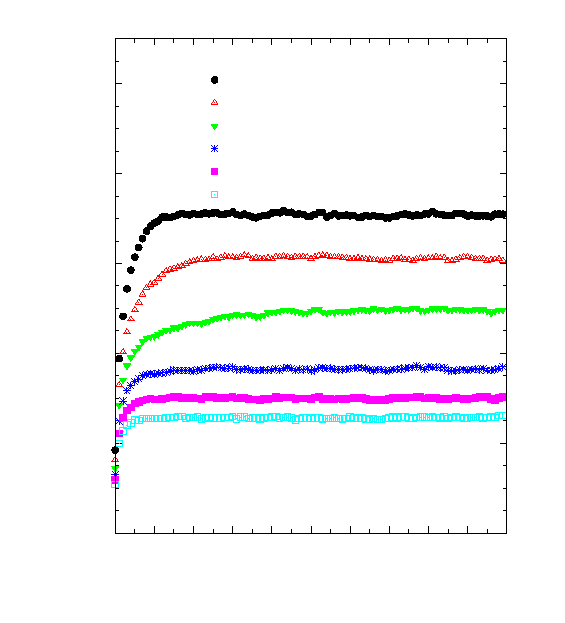
\includegraphics{comparisoncreutzreport}}%
    \gplfronttext
  \end{picture}%
\endgroup

\caption[Behaviour of the plaquette for SU(2)]{Behaviour of the average plaquette during thermalisation for SU(2)}
\label{fig:comparisoncreutz}
\end{figure} 

%-average value of plaquette against number of steps for SU(2)->comparison to \citet{creutzsu2}, one picture

\begin{figure}
	\centering
	% GNUPLOT: LaTeX picture with Postscript
\begingroup
  \makeatletter
  \providecommand\color[2][]{%
    \GenericError{(gnuplot) \space\space\space\@spaces}{%
      Package color not loaded in conjunction with
      terminal option `colourtext'%
    }{See the gnuplot documentation for explanation.%
    }{Either use 'blacktext' in gnuplot or load the package
      color.sty in LaTeX.}%
    \renewcommand\color[2][]{}%
  }%
  \providecommand\includegraphics[2][]{%
    \GenericError{(gnuplot) \space\space\space\@spaces}{%
      Package graphicx or graphics not loaded%
    }{See the gnuplot documentation for explanation.%
    }{The gnuplot epslatex terminal needs graphicx.sty or graphics.sty.}%
    \renewcommand\includegraphics[2][]{}%
  }%
  \providecommand\rotatebox[2]{#2}%
  \@ifundefined{ifGPcolor}{%
    \newif\ifGPcolor
    \GPcolortrue
  }{}%
  \@ifundefined{ifGPblacktext}{%
    \newif\ifGPblacktext
    \GPblacktextfalse
  }{}%
  % define a \g@addto@macro without @ in the name:
  \let\gplgaddtomacro\g@addto@macro
  % define empty templates for all commands taking text:
  \gdef\gplbacktext{}%
  \gdef\gplfronttext{}%
  \makeatother
  \ifGPblacktext
    % no textcolor at all
    \def\colorrgb#1{}%
    \def\colorgray#1{}%
  \else
    % gray or color?
    \ifGPcolor
      \def\colorrgb#1{\color[rgb]{#1}}%
      \def\colorgray#1{\color[gray]{#1}}%
      \expandafter\def\csname LTw\endcsname{\color{white}}%
      \expandafter\def\csname LTb\endcsname{\color{black}}%
      \expandafter\def\csname LTa\endcsname{\color{black}}%
      \expandafter\def\csname LT0\endcsname{\color[rgb]{1,0,0}}%
      \expandafter\def\csname LT1\endcsname{\color[rgb]{0,1,0}}%
      \expandafter\def\csname LT2\endcsname{\color[rgb]{0,0,1}}%
      \expandafter\def\csname LT3\endcsname{\color[rgb]{1,0,1}}%
      \expandafter\def\csname LT4\endcsname{\color[rgb]{0,1,1}}%
      \expandafter\def\csname LT5\endcsname{\color[rgb]{1,1,0}}%
      \expandafter\def\csname LT6\endcsname{\color[rgb]{0,0,0}}%
      \expandafter\def\csname LT7\endcsname{\color[rgb]{1,0.3,0}}%
      \expandafter\def\csname LT8\endcsname{\color[rgb]{0.5,0.5,0.5}}%
    \else
      % gray
      \def\colorrgb#1{\color{black}}%
      \def\colorgray#1{\color[gray]{#1}}%
      \expandafter\def\csname LTw\endcsname{\color{white}}%
      \expandafter\def\csname LTb\endcsname{\color{black}}%
      \expandafter\def\csname LTa\endcsname{\color{black}}%
      \expandafter\def\csname LT0\endcsname{\color{black}}%
      \expandafter\def\csname LT1\endcsname{\color{black}}%
      \expandafter\def\csname LT2\endcsname{\color{black}}%
      \expandafter\def\csname LT3\endcsname{\color{black}}%
      \expandafter\def\csname LT4\endcsname{\color{black}}%
      \expandafter\def\csname LT5\endcsname{\color{black}}%
      \expandafter\def\csname LT6\endcsname{\color{black}}%
      \expandafter\def\csname LT7\endcsname{\color{black}}%
      \expandafter\def\csname LT8\endcsname{\color{black}}%
    \fi
  \fi
    \setlength{\unitlength}{0.0500bp}%
    \ifx\gptboxheight\undefined%
      \newlength{\gptboxheight}%
      \newlength{\gptboxwidth}%
      \newsavebox{\gptboxtext}%
    \fi%
    \setlength{\fboxrule}{0.5pt}%
    \setlength{\fboxsep}{1pt}%
\begin{picture}(5102.00,4534.00)%
    \gplgaddtomacro\gplbacktext{%
      \csname LTb\endcsname%
      \put(814,704){\makebox(0,0)[r]{\strut{}$0.4$}}%
      \put(814,1417){\makebox(0,0)[r]{\strut{}$0.5$}}%
      \put(814,2130){\makebox(0,0)[r]{\strut{}$0.6$}}%
      \put(814,2843){\makebox(0,0)[r]{\strut{}$0.7$}}%
      \put(814,3556){\makebox(0,0)[r]{\strut{}$0.8$}}%
      \put(814,4269){\makebox(0,0)[r]{\strut{}$0.9$}}%
      \put(946,484){\makebox(0,0){\strut{}$0$}}%
      \put(1698,484){\makebox(0,0){\strut{}$100$}}%
      \put(2450,484){\makebox(0,0){\strut{}$200$}}%
      \put(3201,484){\makebox(0,0){\strut{}$300$}}%
      \put(3953,484){\makebox(0,0){\strut{}$400$}}%
      \put(4705,484){\makebox(0,0){\strut{}$500$}}%
    }%
    \gplgaddtomacro\gplfronttext{%
      \csname LTb\endcsname%
      \put(176,2486){\rotatebox{-270}{\makebox(0,0){\strut{}$\langle P\rangle$}}}%
      \put(2825,154){\makebox(0,0){\strut{}steps}}%
      \put(3815,4096){\makebox(0,0){\strut{}}}%
      \csname LTb\endcsname%
      \put(3718,4096){\makebox(0,0)[r]{\strut{}$\beta=5.5$}}%
    }%
    \gplbacktext
    \put(0,0){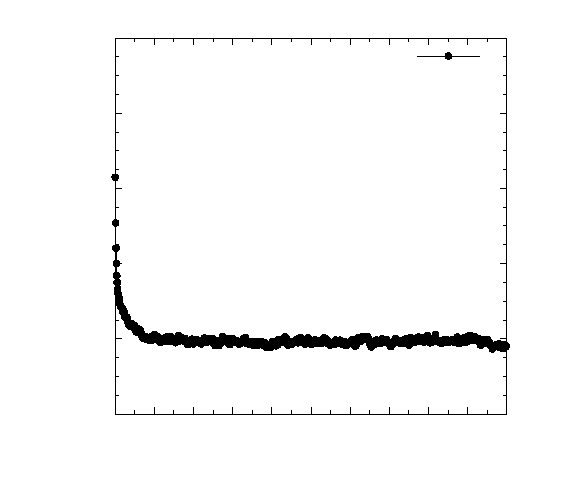
\includegraphics{su3plaquettereport}}%
    \gplfronttext
  \end{picture}%
\endgroup

	\caption[Behaviour of the plaquette for SU(3)]{Behaviour of the average plaquette during thermalisation for SU(3), $\beta=5.5$}
	\label{fig:plaquettethermsu3}
\end{figure} 

The average value for the plaquette during thermalisation is plotted in fig.~\ref{fig:comparisoncreutz} for SU(2)-matrices, from a cold start, i.\,e.\, the entire lattice starting with unity matrices, and in fig.~\ref{fig:plaquettethermsu3} for SU(3) and a hot start. In order to be able to compare our results to the different definition of the plaquette of \citet{creutzsu2}, we plot $1-\langle P\rangle$. Per step, we do 10 Metropolis-updates of each link in the lattice, and the plaquette is calculated directly after one update. The contribution for each link $U_\mu(x)$ is calculated as $\sum_{\mu>\nu}P_{\mu\nu}(x)$.

%-autocorrelation, maybe one picture

%-W(r,t) for different t, one picture


\begin{figure}
	\centering
	% GNUPLOT: LaTeX picture with Postscript
\begingroup
  \makeatletter
  \providecommand\color[2][]{%
    \GenericError{(gnuplot) \space\space\space\@spaces}{%
      Package color not loaded in conjunction with
      terminal option `colourtext'%
    }{See the gnuplot documentation for explanation.%
    }{Either use 'blacktext' in gnuplot or load the package
      color.sty in LaTeX.}%
    \renewcommand\color[2][]{}%
  }%
  \providecommand\includegraphics[2][]{%
    \GenericError{(gnuplot) \space\space\space\@spaces}{%
      Package graphicx or graphics not loaded%
    }{See the gnuplot documentation for explanation.%
    }{The gnuplot epslatex terminal needs graphicx.sty or graphics.sty.}%
    \renewcommand\includegraphics[2][]{}%
  }%
  \providecommand\rotatebox[2]{#2}%
  \@ifundefined{ifGPcolor}{%
    \newif\ifGPcolor
    \GPcolortrue
  }{}%
  \@ifundefined{ifGPblacktext}{%
    \newif\ifGPblacktext
    \GPblacktextfalse
  }{}%
  % define a \g@addto@macro without @ in the name:
  \let\gplgaddtomacro\g@addto@macro
  % define empty templates for all commands taking text:
  \gdef\gplbacktext{}%
  \gdef\gplfronttext{}%
  \makeatother
  \ifGPblacktext
    % no textcolor at all
    \def\colorrgb#1{}%
    \def\colorgray#1{}%
  \else
    % gray or color?
    \ifGPcolor
      \def\colorrgb#1{\color[rgb]{#1}}%
      \def\colorgray#1{\color[gray]{#1}}%
      \expandafter\def\csname LTw\endcsname{\color{white}}%
      \expandafter\def\csname LTb\endcsname{\color{black}}%
      \expandafter\def\csname LTa\endcsname{\color{black}}%
      \expandafter\def\csname LT0\endcsname{\color[rgb]{1,0,0}}%
      \expandafter\def\csname LT1\endcsname{\color[rgb]{0,1,0}}%
      \expandafter\def\csname LT2\endcsname{\color[rgb]{0,0,1}}%
      \expandafter\def\csname LT3\endcsname{\color[rgb]{1,0,1}}%
      \expandafter\def\csname LT4\endcsname{\color[rgb]{0,1,1}}%
      \expandafter\def\csname LT5\endcsname{\color[rgb]{1,1,0}}%
      \expandafter\def\csname LT6\endcsname{\color[rgb]{0,0,0}}%
      \expandafter\def\csname LT7\endcsname{\color[rgb]{1,0.3,0}}%
      \expandafter\def\csname LT8\endcsname{\color[rgb]{0.5,0.5,0.5}}%
    \else
      % gray
      \def\colorrgb#1{\color{black}}%
      \def\colorgray#1{\color[gray]{#1}}%
      \expandafter\def\csname LTw\endcsname{\color{white}}%
      \expandafter\def\csname LTb\endcsname{\color{black}}%
      \expandafter\def\csname LTa\endcsname{\color{black}}%
      \expandafter\def\csname LT0\endcsname{\color{black}}%
      \expandafter\def\csname LT1\endcsname{\color{black}}%
      \expandafter\def\csname LT2\endcsname{\color{black}}%
      \expandafter\def\csname LT3\endcsname{\color{black}}%
      \expandafter\def\csname LT4\endcsname{\color{black}}%
      \expandafter\def\csname LT5\endcsname{\color{black}}%
      \expandafter\def\csname LT6\endcsname{\color{black}}%
      \expandafter\def\csname LT7\endcsname{\color{black}}%
      \expandafter\def\csname LT8\endcsname{\color{black}}%
    \fi
  \fi
    \setlength{\unitlength}{0.0500bp}%
    \ifx\gptboxheight\undefined%
      \newlength{\gptboxheight}%
      \newlength{\gptboxwidth}%
      \newsavebox{\gptboxtext}%
    \fi%
    \setlength{\fboxrule}{0.5pt}%
    \setlength{\fboxsep}{1pt}%
\begin{picture}(5102.00,5668.00)%
    \gplgaddtomacro\gplbacktext{%
      \csname LTb\endcsname%
      \put(814,704){\makebox(0,0)[r]{\strut{}$0.1$}}%
      \put(814,1291){\makebox(0,0)[r]{\strut{}$0.2$}}%
      \put(814,1879){\makebox(0,0)[r]{\strut{}$0.3$}}%
      \put(814,2466){\makebox(0,0)[r]{\strut{}$0.4$}}%
      \put(814,3054){\makebox(0,0)[r]{\strut{}$0.5$}}%
      \put(814,3641){\makebox(0,0)[r]{\strut{}$0.6$}}%
      \put(814,4228){\makebox(0,0)[r]{\strut{}$0.7$}}%
      \put(814,4816){\makebox(0,0)[r]{\strut{}$0.8$}}%
      \put(814,5403){\makebox(0,0)[r]{\strut{}$0.9$}}%
      \put(946,484){\makebox(0,0){\strut{}$1.5$}}%
      \put(1416,484){\makebox(0,0){\strut{}$2$}}%
      \put(1886,484){\makebox(0,0){\strut{}$2.5$}}%
      \put(2356,484){\makebox(0,0){\strut{}$3$}}%
      \put(2826,484){\makebox(0,0){\strut{}$3.5$}}%
      \put(3295,484){\makebox(0,0){\strut{}$4$}}%
      \put(3765,484){\makebox(0,0){\strut{}$4.5$}}%
      \put(4235,484){\makebox(0,0){\strut{}$5$}}%
      \put(4705,484){\makebox(0,0){\strut{}$5.5$}}%
    }%
    \gplgaddtomacro\gplfronttext{%
      \csname LTb\endcsname%
      \put(176,3053){\rotatebox{-270}{\makebox(0,0){\strut{}$\langle P\rangle$}}}%
      \put(2825,154){\makebox(0,0){\strut{}$\beta$}}%
      \put(1835,5230){\makebox(0,0){\strut{}}}%
      \csname LTb\endcsname%
      \put(1738,5230){\makebox(0,0)[r]{\strut{}SU(2)}}%
      \csname LTb\endcsname%
      \put(1738,5010){\makebox(0,0)[r]{\strut{}SU(3)}}%
    }%
    \gplbacktext
    \put(0,0){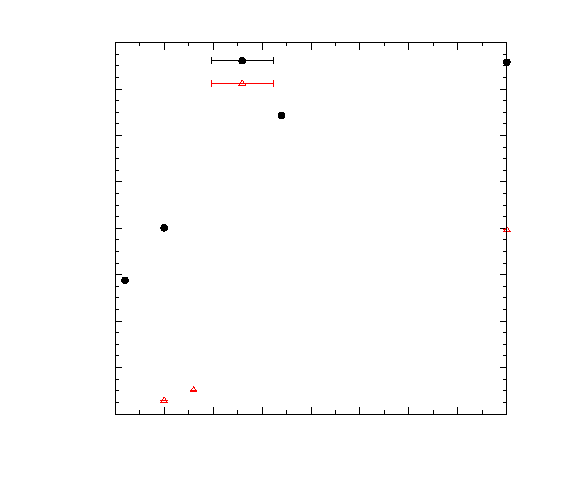
\includegraphics{plaquettereport}}%
    \gplfronttext
  \end{picture}%
\endgroup

	\caption[Mean values of the plaquette]{Mean values of the plaquette for SU(2) and SU(3) for different $\beta$. The relative error is $10^{-5}$ or smaller.}
	\label{fig:plaquettetotal}
\end{figure}

After the thermalisation, we do our measurements on the lattice. All measurements are done after at least 100 thermalisation steps, with the number of measurements between $2048$ and $8192$ per $\beta$. The analysis is done with a binsize of $32$ and $200$ bootstrapsamples. 

The average plaquette for different $\beta$ and SU(2) and SU(3) is shown in fig.~\ref{fig:plaquettetotal}. Here we measure the plaquette by calculating $\sum_{\mu>\nu}P_{\mu\nu}(x)$ for each lattice site $x$, and also plot the expectations for strong and weak coupling in SU(2) as given by \citet{creutzsu2}.

\begin{figure}
	\centering
	% GNUPLOT: LaTeX picture with Postscript
\begingroup
  \makeatletter
  \providecommand\color[2][]{%
    \GenericError{(gnuplot) \space\space\space\@spaces}{%
      Package color not loaded in conjunction with
      terminal option `colourtext'%
    }{See the gnuplot documentation for explanation.%
    }{Either use 'blacktext' in gnuplot or load the package
      color.sty in LaTeX.}%
    \renewcommand\color[2][]{}%
  }%
  \providecommand\includegraphics[2][]{%
    \GenericError{(gnuplot) \space\space\space\@spaces}{%
      Package graphicx or graphics not loaded%
    }{See the gnuplot documentation for explanation.%
    }{The gnuplot epslatex terminal needs graphicx.sty or graphics.sty.}%
    \renewcommand\includegraphics[2][]{}%
  }%
  \providecommand\rotatebox[2]{#2}%
  \@ifundefined{ifGPcolor}{%
    \newif\ifGPcolor
    \GPcolortrue
  }{}%
  \@ifundefined{ifGPblacktext}{%
    \newif\ifGPblacktext
    \GPblacktextfalse
  }{}%
  % define a \g@addto@macro without @ in the name:
  \let\gplgaddtomacro\g@addto@macro
  % define empty templates for all commands taking text:
  \gdef\gplbacktext{}%
  \gdef\gplfronttext{}%
  \makeatother
  \ifGPblacktext
    % no textcolor at all
    \def\colorrgb#1{}%
    \def\colorgray#1{}%
  \else
    % gray or color?
    \ifGPcolor
      \def\colorrgb#1{\color[rgb]{#1}}%
      \def\colorgray#1{\color[gray]{#1}}%
      \expandafter\def\csname LTw\endcsname{\color{white}}%
      \expandafter\def\csname LTb\endcsname{\color{black}}%
      \expandafter\def\csname LTa\endcsname{\color{black}}%
      \expandafter\def\csname LT0\endcsname{\color[rgb]{1,0,0}}%
      \expandafter\def\csname LT1\endcsname{\color[rgb]{0,1,0}}%
      \expandafter\def\csname LT2\endcsname{\color[rgb]{0,0,1}}%
      \expandafter\def\csname LT3\endcsname{\color[rgb]{1,0,1}}%
      \expandafter\def\csname LT4\endcsname{\color[rgb]{0,1,1}}%
      \expandafter\def\csname LT5\endcsname{\color[rgb]{1,1,0}}%
      \expandafter\def\csname LT6\endcsname{\color[rgb]{0,0,0}}%
      \expandafter\def\csname LT7\endcsname{\color[rgb]{1,0.3,0}}%
      \expandafter\def\csname LT8\endcsname{\color[rgb]{0.5,0.5,0.5}}%
    \else
      % gray
      \def\colorrgb#1{\color{black}}%
      \def\colorgray#1{\color[gray]{#1}}%
      \expandafter\def\csname LTw\endcsname{\color{white}}%
      \expandafter\def\csname LTb\endcsname{\color{black}}%
      \expandafter\def\csname LTa\endcsname{\color{black}}%
      \expandafter\def\csname LT0\endcsname{\color{black}}%
      \expandafter\def\csname LT1\endcsname{\color{black}}%
      \expandafter\def\csname LT2\endcsname{\color{black}}%
      \expandafter\def\csname LT3\endcsname{\color{black}}%
      \expandafter\def\csname LT4\endcsname{\color{black}}%
      \expandafter\def\csname LT5\endcsname{\color{black}}%
      \expandafter\def\csname LT6\endcsname{\color{black}}%
      \expandafter\def\csname LT7\endcsname{\color{black}}%
      \expandafter\def\csname LT8\endcsname{\color{black}}%
    \fi
  \fi
    \setlength{\unitlength}{0.0500bp}%
    \ifx\gptboxheight\undefined%
      \newlength{\gptboxheight}%
      \newlength{\gptboxwidth}%
      \newsavebox{\gptboxtext}%
    \fi%
    \setlength{\fboxrule}{0.5pt}%
    \setlength{\fboxsep}{1pt}%
\begin{picture}(5102.00,4534.00)%
    \gplgaddtomacro\gplbacktext{%
      \csname LTb\endcsname%
      \put(946,704){\makebox(0,0)[r]{\strut{}$0$}}%
      \put(946,1061){\makebox(0,0)[r]{\strut{}$0.05$}}%
      \put(946,1417){\makebox(0,0)[r]{\strut{}$0.1$}}%
      \put(946,1774){\makebox(0,0)[r]{\strut{}$0.15$}}%
      \put(946,2130){\makebox(0,0)[r]{\strut{}$0.2$}}%
      \put(946,2487){\makebox(0,0)[r]{\strut{}$0.25$}}%
      \put(946,2843){\makebox(0,0)[r]{\strut{}$0.3$}}%
      \put(946,3200){\makebox(0,0)[r]{\strut{}$0.35$}}%
      \put(946,3556){\makebox(0,0)[r]{\strut{}$0.4$}}%
      \put(946,3912){\makebox(0,0)[r]{\strut{}$0.45$}}%
      \put(946,4269){\makebox(0,0)[r]{\strut{}$0.5$}}%
      \put(1078,484){\makebox(0,0){\strut{}$1$}}%
      \put(1683,484){\makebox(0,0){\strut{}$1.5$}}%
      \put(2287,484){\makebox(0,0){\strut{}$2$}}%
      \put(2892,484){\makebox(0,0){\strut{}$2.5$}}%
      \put(3496,484){\makebox(0,0){\strut{}$3$}}%
      \put(4101,484){\makebox(0,0){\strut{}$3.5$}}%
      \put(4705,484){\makebox(0,0){\strut{}$4$}}%
    }%
    \gplgaddtomacro\gplfronttext{%
      \csname LTb\endcsname%
      \put(176,2486){\rotatebox{-270}{\makebox(0,0){\strut{}$W(R/a, T/a)$}}}%
      \put(2891,154){\makebox(0,0){\strut{}$T/a$}}%
      \put(3947,4096){\makebox(0,0){\strut{}}}%
      \csname LTb\endcsname%
      \put(3718,4096){\makebox(0,0)[r]{\strut{}R=1}}%
      \csname LTb\endcsname%
      \put(3718,3876){\makebox(0,0)[r]{\strut{}R=2}}%
      \csname LTb\endcsname%
      \put(3718,3656){\makebox(0,0)[r]{\strut{}R=3}}%
      \csname LTb\endcsname%
      \put(3718,3436){\makebox(0,0)[r]{\strut{}R=4}}%
    }%
    \gplbacktext
    \put(0,0){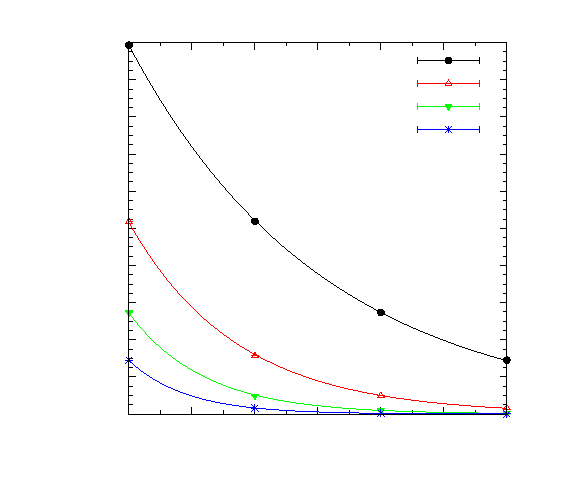
\includegraphics{wilsonloopsu3beta55report}}%
    \gplfronttext
  \end{picture}%
\endgroup

	\caption[Different Wilson loops for SU(3), $\beta=5.5$]{Wilson loops for several $R$ and $T$ including fits to a falling exponential function for SU(3), $\beta=5.5$. The errors too small too be visible.}
	\label{fig:wilsonloopbeta5.5su3}
\end{figure} 

We measure the Wilson-loops for $R=(1,2,3,4)$ and $T=(1,2,3,4)$ for all points in the lattice. For each $\beta$, we fit falling exponential curves to the datasets for constant $R$ and varying $T$. One such dataset with fits is shown in fig.~\ref{fig:wilsonloopbeta5.5su3}. For all fits we use the nonlinear least-squares Marquardt-Levenberg algorithm built into gnuplot (\citet{gnuplotdoc}).

%how to extract V(r) from W(r). fit values: maybe in appendix?


\begin{figure}
	\centering
	% GNUPLOT: LaTeX picture with Postscript
\begingroup
  \makeatletter
  \providecommand\color[2][]{%
    \GenericError{(gnuplot) \space\space\space\@spaces}{%
      Package color not loaded in conjunction with
      terminal option `colourtext'%
    }{See the gnuplot documentation for explanation.%
    }{Either use 'blacktext' in gnuplot or load the package
      color.sty in LaTeX.}%
    \renewcommand\color[2][]{}%
  }%
  \providecommand\includegraphics[2][]{%
    \GenericError{(gnuplot) \space\space\space\@spaces}{%
      Package graphicx or graphics not loaded%
    }{See the gnuplot documentation for explanation.%
    }{The gnuplot epslatex terminal needs graphicx.sty or graphics.sty.}%
    \renewcommand\includegraphics[2][]{}%
  }%
  \providecommand\rotatebox[2]{#2}%
  \@ifundefined{ifGPcolor}{%
    \newif\ifGPcolor
    \GPcolortrue
  }{}%
  \@ifundefined{ifGPblacktext}{%
    \newif\ifGPblacktext
    \GPblacktextfalse
  }{}%
  % define a \g@addto@macro without @ in the name:
  \let\gplgaddtomacro\g@addto@macro
  % define empty templates for all commands taking text:
  \gdef\gplbacktext{}%
  \gdef\gplfronttext{}%
  \makeatother
  \ifGPblacktext
    % no textcolor at all
    \def\colorrgb#1{}%
    \def\colorgray#1{}%
  \else
    % gray or color?
    \ifGPcolor
      \def\colorrgb#1{\color[rgb]{#1}}%
      \def\colorgray#1{\color[gray]{#1}}%
      \expandafter\def\csname LTw\endcsname{\color{white}}%
      \expandafter\def\csname LTb\endcsname{\color{black}}%
      \expandafter\def\csname LTa\endcsname{\color{black}}%
      \expandafter\def\csname LT0\endcsname{\color[rgb]{1,0,0}}%
      \expandafter\def\csname LT1\endcsname{\color[rgb]{0,1,0}}%
      \expandafter\def\csname LT2\endcsname{\color[rgb]{0,0,1}}%
      \expandafter\def\csname LT3\endcsname{\color[rgb]{1,0,1}}%
      \expandafter\def\csname LT4\endcsname{\color[rgb]{0,1,1}}%
      \expandafter\def\csname LT5\endcsname{\color[rgb]{1,1,0}}%
      \expandafter\def\csname LT6\endcsname{\color[rgb]{0,0,0}}%
      \expandafter\def\csname LT7\endcsname{\color[rgb]{1,0.3,0}}%
      \expandafter\def\csname LT8\endcsname{\color[rgb]{0.5,0.5,0.5}}%
    \else
      % gray
      \def\colorrgb#1{\color{black}}%
      \def\colorgray#1{\color[gray]{#1}}%
      \expandafter\def\csname LTw\endcsname{\color{white}}%
      \expandafter\def\csname LTb\endcsname{\color{black}}%
      \expandafter\def\csname LTa\endcsname{\color{black}}%
      \expandafter\def\csname LT0\endcsname{\color{black}}%
      \expandafter\def\csname LT1\endcsname{\color{black}}%
      \expandafter\def\csname LT2\endcsname{\color{black}}%
      \expandafter\def\csname LT3\endcsname{\color{black}}%
      \expandafter\def\csname LT4\endcsname{\color{black}}%
      \expandafter\def\csname LT5\endcsname{\color{black}}%
      \expandafter\def\csname LT6\endcsname{\color{black}}%
      \expandafter\def\csname LT7\endcsname{\color{black}}%
      \expandafter\def\csname LT8\endcsname{\color{black}}%
    \fi
  \fi
    \setlength{\unitlength}{0.0500bp}%
    \ifx\gptboxheight\undefined%
      \newlength{\gptboxheight}%
      \newlength{\gptboxwidth}%
      \newsavebox{\gptboxtext}%
    \fi%
    \setlength{\fboxrule}{0.5pt}%
    \setlength{\fboxsep}{1pt}%
\begin{picture}(5102.00,4534.00)%
    \gplgaddtomacro\gplbacktext{%
      \csname LTb\endcsname%
      \put(814,704){\makebox(0,0)[r]{\strut{}$0$}}%
      \put(814,1150){\makebox(0,0)[r]{\strut{}$0.5$}}%
      \put(814,1595){\makebox(0,0)[r]{\strut{}$1$}}%
      \put(814,2041){\makebox(0,0)[r]{\strut{}$1.5$}}%
      \put(814,2487){\makebox(0,0)[r]{\strut{}$2$}}%
      \put(814,2932){\makebox(0,0)[r]{\strut{}$2.5$}}%
      \put(814,3378){\makebox(0,0)[r]{\strut{}$3$}}%
      \put(814,3823){\makebox(0,0)[r]{\strut{}$3.5$}}%
      \put(814,4269){\makebox(0,0)[r]{\strut{}$4$}}%
      \put(946,484){\makebox(0,0){\strut{}$0.5$}}%
      \put(1364,484){\makebox(0,0){\strut{}$1$}}%
      \put(1781,484){\makebox(0,0){\strut{}$1.5$}}%
      \put(2199,484){\makebox(0,0){\strut{}$2$}}%
      \put(2617,484){\makebox(0,0){\strut{}$2.5$}}%
      \put(3034,484){\makebox(0,0){\strut{}$3$}}%
      \put(3452,484){\makebox(0,0){\strut{}$3.5$}}%
      \put(3870,484){\makebox(0,0){\strut{}$4$}}%
      \put(4287,484){\makebox(0,0){\strut{}$4.5$}}%
      \put(4705,484){\makebox(0,0){\strut{}$5$}}%
    }%
    \gplgaddtomacro\gplfronttext{%
      \csname LTb\endcsname%
      \put(176,2486){\rotatebox{-270}{\makebox(0,0){\strut{}$aV(R/a)$}}}%
      \put(2825,154){\makebox(0,0){\strut{}$R/a$}}%
      \put(1835,4096){\makebox(0,0){\strut{}}}%
      \csname LTb\endcsname%
      \put(1738,4096){\makebox(0,0)[r]{\strut{}$\beta=$1.6}}%
      \csname LTb\endcsname%
      \put(1738,3876){\makebox(0,0)[r]{\strut{}$\beta=$2.0}}%
      \csname LTb\endcsname%
      \put(1738,3656){\makebox(0,0)[r]{\strut{}$\beta=$2.6}}%
      \csname LTb\endcsname%
      \put(1738,3436){\makebox(0,0)[r]{\strut{}$\beta=$3.2}}%
      \csname LTb\endcsname%
      \put(1738,3216){\makebox(0,0)[r]{\strut{}$\beta=$4.2}}%
      \csname LTb\endcsname%
      \put(1738,2996){\makebox(0,0)[r]{\strut{}$\beta=$5.5}}%
    }%
    \gplbacktext
    \put(0,0){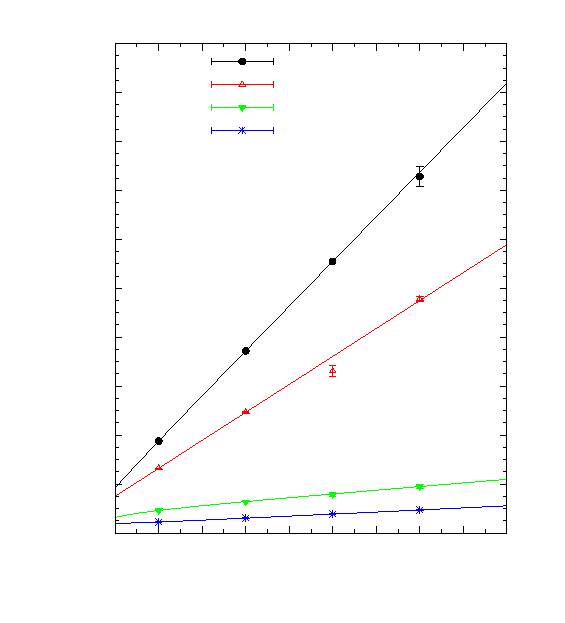
\includegraphics{potentialsu2report}}%
    \gplfronttext
  \end{picture}%
\endgroup

	\caption[Potentials obtained using SU(2)]{Potential values obtained from fitting to the Wilson loops and fit to potential for SU(2)}
	\label{fig:fittedpotentialssu2}
\end{figure} 


\begin{figure}
	\centering
	% GNUPLOT: LaTeX picture with Postscript
\begingroup
  \makeatletter
  \providecommand\color[2][]{%
    \GenericError{(gnuplot) \space\space\space\@spaces}{%
      Package color not loaded in conjunction with
      terminal option `colourtext'%
    }{See the gnuplot documentation for explanation.%
    }{Either use 'blacktext' in gnuplot or load the package
      color.sty in LaTeX.}%
    \renewcommand\color[2][]{}%
  }%
  \providecommand\includegraphics[2][]{%
    \GenericError{(gnuplot) \space\space\space\@spaces}{%
      Package graphicx or graphics not loaded%
    }{See the gnuplot documentation for explanation.%
    }{The gnuplot epslatex terminal needs graphicx.sty or graphics.sty.}%
    \renewcommand\includegraphics[2][]{}%
  }%
  \providecommand\rotatebox[2]{#2}%
  \@ifundefined{ifGPcolor}{%
    \newif\ifGPcolor
    \GPcolortrue
  }{}%
  \@ifundefined{ifGPblacktext}{%
    \newif\ifGPblacktext
    \GPblacktextfalse
  }{}%
  % define a \g@addto@macro without @ in the name:
  \let\gplgaddtomacro\g@addto@macro
  % define empty templates for all commands taking text:
  \gdef\gplbacktext{}%
  \gdef\gplfronttext{}%
  \makeatother
  \ifGPblacktext
    % no textcolor at all
    \def\colorrgb#1{}%
    \def\colorgray#1{}%
  \else
    % gray or color?
    \ifGPcolor
      \def\colorrgb#1{\color[rgb]{#1}}%
      \def\colorgray#1{\color[gray]{#1}}%
      \expandafter\def\csname LTw\endcsname{\color{white}}%
      \expandafter\def\csname LTb\endcsname{\color{black}}%
      \expandafter\def\csname LTa\endcsname{\color{black}}%
      \expandafter\def\csname LT0\endcsname{\color[rgb]{1,0,0}}%
      \expandafter\def\csname LT1\endcsname{\color[rgb]{0,1,0}}%
      \expandafter\def\csname LT2\endcsname{\color[rgb]{0,0,1}}%
      \expandafter\def\csname LT3\endcsname{\color[rgb]{1,0,1}}%
      \expandafter\def\csname LT4\endcsname{\color[rgb]{0,1,1}}%
      \expandafter\def\csname LT5\endcsname{\color[rgb]{1,1,0}}%
      \expandafter\def\csname LT6\endcsname{\color[rgb]{0,0,0}}%
      \expandafter\def\csname LT7\endcsname{\color[rgb]{1,0.3,0}}%
      \expandafter\def\csname LT8\endcsname{\color[rgb]{0.5,0.5,0.5}}%
    \else
      % gray
      \def\colorrgb#1{\color{black}}%
      \def\colorgray#1{\color[gray]{#1}}%
      \expandafter\def\csname LTw\endcsname{\color{white}}%
      \expandafter\def\csname LTb\endcsname{\color{black}}%
      \expandafter\def\csname LTa\endcsname{\color{black}}%
      \expandafter\def\csname LT0\endcsname{\color{black}}%
      \expandafter\def\csname LT1\endcsname{\color{black}}%
      \expandafter\def\csname LT2\endcsname{\color{black}}%
      \expandafter\def\csname LT3\endcsname{\color{black}}%
      \expandafter\def\csname LT4\endcsname{\color{black}}%
      \expandafter\def\csname LT5\endcsname{\color{black}}%
      \expandafter\def\csname LT6\endcsname{\color{black}}%
      \expandafter\def\csname LT7\endcsname{\color{black}}%
      \expandafter\def\csname LT8\endcsname{\color{black}}%
    \fi
  \fi
    \setlength{\unitlength}{0.0500bp}%
    \ifx\gptboxheight\undefined%
      \newlength{\gptboxheight}%
      \newlength{\gptboxwidth}%
      \newsavebox{\gptboxtext}%
    \fi%
    \setlength{\fboxrule}{0.5pt}%
    \setlength{\fboxsep}{1pt}%
\begin{picture}(5102.00,4534.00)%
    \gplgaddtomacro\gplbacktext{%
      \csname LTb\endcsname%
      \put(682,704){\makebox(0,0)[r]{\strut{}$-1$}}%
      \put(682,1061){\makebox(0,0)[r]{\strut{}$0$}}%
      \put(682,1417){\makebox(0,0)[r]{\strut{}$1$}}%
      \put(682,1774){\makebox(0,0)[r]{\strut{}$2$}}%
      \put(682,2130){\makebox(0,0)[r]{\strut{}$3$}}%
      \put(682,2487){\makebox(0,0)[r]{\strut{}$4$}}%
      \put(682,2843){\makebox(0,0)[r]{\strut{}$5$}}%
      \put(682,3200){\makebox(0,0)[r]{\strut{}$6$}}%
      \put(682,3556){\makebox(0,0)[r]{\strut{}$7$}}%
      \put(682,3913){\makebox(0,0)[r]{\strut{}$8$}}%
      \put(682,4269){\makebox(0,0)[r]{\strut{}$9$}}%
      \put(814,484){\makebox(0,0){\strut{}$0.5$}}%
      \put(1246,484){\makebox(0,0){\strut{}$1$}}%
      \put(1679,484){\makebox(0,0){\strut{}$1.5$}}%
      \put(2111,484){\makebox(0,0){\strut{}$2$}}%
      \put(2543,484){\makebox(0,0){\strut{}$2.5$}}%
      \put(2976,484){\makebox(0,0){\strut{}$3$}}%
      \put(3408,484){\makebox(0,0){\strut{}$3.5$}}%
      \put(3840,484){\makebox(0,0){\strut{}$4$}}%
      \put(4273,484){\makebox(0,0){\strut{}$4.5$}}%
      \put(4705,484){\makebox(0,0){\strut{}$5$}}%
    }%
    \gplgaddtomacro\gplfronttext{%
      \csname LTb\endcsname%
      \put(176,2486){\rotatebox{-270}{\makebox(0,0){\strut{}$aV(R/a)$}}}%
      \put(2759,154){\makebox(0,0){\strut{}$R/a$}}%
      \put(1703,4096){\makebox(0,0){\strut{}}}%
      \csname LTb\endcsname%
      \put(1606,4096){\makebox(0,0)[r]{\strut{}$\beta=$2.3}}%
      \csname LTb\endcsname%
      \put(1606,3876){\makebox(0,0)[r]{\strut{}$\beta=$3.0}}%
      \csname LTb\endcsname%
      \put(1606,3656){\makebox(0,0)[r]{\strut{}$\beta=$3.5}}%
      \csname LTb\endcsname%
      \put(1606,3436){\makebox(0,0)[r]{\strut{}$\beta=$4.0}}%
      \csname LTb\endcsname%
      \put(1606,3216){\makebox(0,0)[r]{\strut{}$\beta=$4.5}}%
      \csname LTb\endcsname%
      \put(1606,2996){\makebox(0,0)[r]{\strut{}$\beta=$5.5}}%
    }%
    \gplbacktext
    \put(0,0){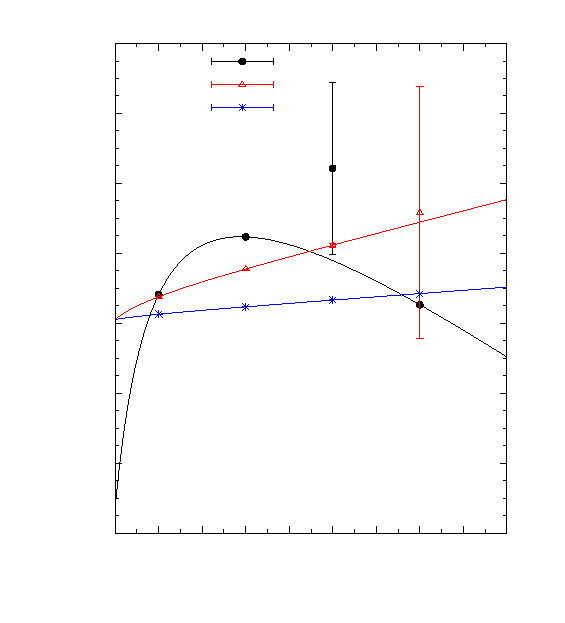
\includegraphics{potentialsu3report}}%
    \gplfronttext
  \end{picture}%
\endgroup

	\caption[Potentials obtained using SU(3)]{Potential values obtained from fitting to the Wilson loops and fit to potential for SU(3)}
	\label{fig:fittedpotentialssu3}
\end{figure} 

We use the parameters obtained from the Wilson-loops as values for the potential $aV(R/a)$. To these points, we fit $aV\left(\frac{R}{a}\right)=a^2\sigma \frac{R}{a}-b\left(\frac{R}{a}\right)^{-1}+ac$. The resulting potentials for SU(2) are shown in fig.~\ref{fig:fittedpotentialssu2}, those for SU(3) in fig.~\ref{fig:fittedpotentialssu3}. We neglect systematic errors arising from the discretization. The resulting potentials for SU(3) for $\beta=2.0$ and $\beta=2.3$ are not plotted or considered further because the fit returns a negative slope.


\begin{figure}
	\centering
	% GNUPLOT: LaTeX picture with Postscript
\begingroup
  \makeatletter
  \providecommand\color[2][]{%
    \GenericError{(gnuplot) \space\space\space\@spaces}{%
      Package color not loaded in conjunction with
      terminal option `colourtext'%
    }{See the gnuplot documentation for explanation.%
    }{Either use 'blacktext' in gnuplot or load the package
      color.sty in LaTeX.}%
    \renewcommand\color[2][]{}%
  }%
  \providecommand\includegraphics[2][]{%
    \GenericError{(gnuplot) \space\space\space\@spaces}{%
      Package graphicx or graphics not loaded%
    }{See the gnuplot documentation for explanation.%
    }{The gnuplot epslatex terminal needs graphicx.sty or graphics.sty.}%
    \renewcommand\includegraphics[2][]{}%
  }%
  \providecommand\rotatebox[2]{#2}%
  \@ifundefined{ifGPcolor}{%
    \newif\ifGPcolor
    \GPcolortrue
  }{}%
  \@ifundefined{ifGPblacktext}{%
    \newif\ifGPblacktext
    \GPblacktextfalse
  }{}%
  % define a \g@addto@macro without @ in the name:
  \let\gplgaddtomacro\g@addto@macro
  % define empty templates for all commands taking text:
  \gdef\gplbacktext{}%
  \gdef\gplfronttext{}%
  \makeatother
  \ifGPblacktext
    % no textcolor at all
    \def\colorrgb#1{}%
    \def\colorgray#1{}%
  \else
    % gray or color?
    \ifGPcolor
      \def\colorrgb#1{\color[rgb]{#1}}%
      \def\colorgray#1{\color[gray]{#1}}%
      \expandafter\def\csname LTw\endcsname{\color{white}}%
      \expandafter\def\csname LTb\endcsname{\color{black}}%
      \expandafter\def\csname LTa\endcsname{\color{black}}%
      \expandafter\def\csname LT0\endcsname{\color[rgb]{1,0,0}}%
      \expandafter\def\csname LT1\endcsname{\color[rgb]{0,1,0}}%
      \expandafter\def\csname LT2\endcsname{\color[rgb]{0,0,1}}%
      \expandafter\def\csname LT3\endcsname{\color[rgb]{1,0,1}}%
      \expandafter\def\csname LT4\endcsname{\color[rgb]{0,1,1}}%
      \expandafter\def\csname LT5\endcsname{\color[rgb]{1,1,0}}%
      \expandafter\def\csname LT6\endcsname{\color[rgb]{0,0,0}}%
      \expandafter\def\csname LT7\endcsname{\color[rgb]{1,0.3,0}}%
      \expandafter\def\csname LT8\endcsname{\color[rgb]{0.5,0.5,0.5}}%
    \else
      % gray
      \def\colorrgb#1{\color{black}}%
      \def\colorgray#1{\color[gray]{#1}}%
      \expandafter\def\csname LTw\endcsname{\color{white}}%
      \expandafter\def\csname LTb\endcsname{\color{black}}%
      \expandafter\def\csname LTa\endcsname{\color{black}}%
      \expandafter\def\csname LT0\endcsname{\color{black}}%
      \expandafter\def\csname LT1\endcsname{\color{black}}%
      \expandafter\def\csname LT2\endcsname{\color{black}}%
      \expandafter\def\csname LT3\endcsname{\color{black}}%
      \expandafter\def\csname LT4\endcsname{\color{black}}%
      \expandafter\def\csname LT5\endcsname{\color{black}}%
      \expandafter\def\csname LT6\endcsname{\color{black}}%
      \expandafter\def\csname LT7\endcsname{\color{black}}%
      \expandafter\def\csname LT8\endcsname{\color{black}}%
    \fi
  \fi
    \setlength{\unitlength}{0.0500bp}%
    \ifx\gptboxheight\undefined%
      \newlength{\gptboxheight}%
      \newlength{\gptboxwidth}%
      \newsavebox{\gptboxtext}%
    \fi%
    \setlength{\fboxrule}{0.5pt}%
    \setlength{\fboxsep}{1pt}%
\begin{picture}(5102.00,4534.00)%
    \gplgaddtomacro\gplbacktext{%
      \csname LTb\endcsname%
      \put(682,704){\makebox(0,0)[r]{\strut{}$-5$}}%
      \put(682,1213){\makebox(0,0)[r]{\strut{}$-4$}}%
      \put(682,1723){\makebox(0,0)[r]{\strut{}$-3$}}%
      \put(682,2232){\makebox(0,0)[r]{\strut{}$-2$}}%
      \put(682,2741){\makebox(0,0)[r]{\strut{}$-1$}}%
      \put(682,3250){\makebox(0,0)[r]{\strut{}$0$}}%
      \put(682,3760){\makebox(0,0)[r]{\strut{}$1$}}%
      \put(682,4269){\makebox(0,0)[r]{\strut{}$2$}}%
      \put(814,484){\makebox(0,0){\strut{}$1.5$}}%
      \put(1300,484){\makebox(0,0){\strut{}$2$}}%
      \put(1787,484){\makebox(0,0){\strut{}$2.5$}}%
      \put(2273,484){\makebox(0,0){\strut{}$3$}}%
      \put(2760,484){\makebox(0,0){\strut{}$3.5$}}%
      \put(3246,484){\makebox(0,0){\strut{}$4$}}%
      \put(3732,484){\makebox(0,0){\strut{}$4.5$}}%
      \put(4219,484){\makebox(0,0){\strut{}$5$}}%
      \put(4705,484){\makebox(0,0){\strut{}$5.5$}}%
    }%
    \gplgaddtomacro\gplfronttext{%
      \csname LTb\endcsname%
      \put(176,2486){\rotatebox{-270}{\makebox(0,0){\strut{}$a^2\sigma$}}}%
      \put(2759,154){\makebox(0,0){\strut{}$\beta$}}%
      \put(1703,4096){\makebox(0,0){\strut{}}}%
      \csname LTb\endcsname%
      \put(1606,4096){\makebox(0,0)[r]{\strut{}SU(2)}}%
      \csname LTb\endcsname%
      \put(1606,3876){\makebox(0,0)[r]{\strut{}SU(3)}}%
    }%
    \gplbacktext
    \put(0,0){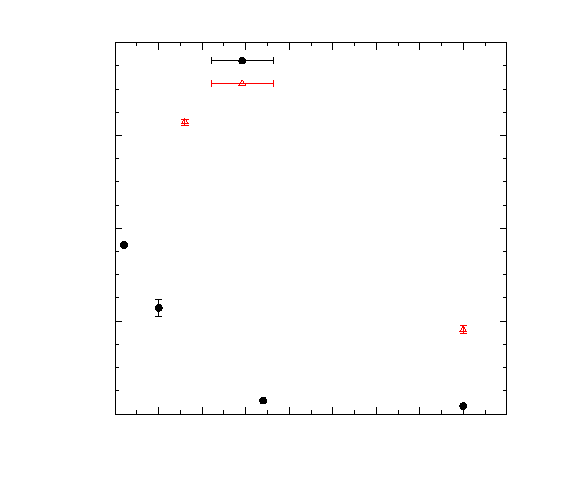
\includegraphics{stringtensionreport}}%
    \gplfronttext
  \end{picture}%
\endgroup

	\caption[String tension obtained from potential]{String tension obtained as the linear slope of the potentials}
	\label{fig:stringtension}
\end{figure}

The linear parts of the potentials correspond to the string tensions, which are shown in fig.~\ref{fig:stringtension}.
%fit to potential, for one temperature each for SU(2) and SU(3)

\section{Discussion}

Comparison of fig.~\ref{fig:comparisoncreutz} with \citet{creutzsu2} shows our values are stabilizing at the same values, so we have implemented the action correctly for SU(2) and can proceed with the rest of our measurements. The same is true for fig.~\ref{fig:plaquettethermsu3}, the plaquette approaches a value of $0.5$ for SU(3), the same as predicted by \citet{lepagelqcd}. 

%Thermalisation of plaquette in SU(2) reproduces \citet{creutzsu2} nicely, average value for $\beta=5.5$ in SU(3) fits well to expectation from \citet{lepagelqcd}.

As can be seen in fig.~\ref{fig:plaquettetotal}, the average
 plaquette rises with $\beta$, i.\,e.\, with smaller coupling. 
For SU(2) the predicted function to reproduce strong coupling holds for $\beta=1.6, 2.0$ and $\beta=2.5$. $\beta=3.2$ seems to be the crossing point towards weak coupling, and for larger values of $\beta$, e.\,g.\, $\beta=5.5$ the function for weak coupling gets closer to the measured values of the plaquette.

The exponential decay of the Wilson Loop with distance in time can be nicely seen in fig.~\ref{fig:wilsonloopbeta5.5su3}, and is observed for all datasets. For some parameter combinations there are problems fitting an exponential curve because of negative values for the Wilson loop, which arise from statistical fluctuations.

%Most Wilson-loops have ncie exponential curves, however some problems with negative values for large $R$. 

Overall the fitted values for the potential reproduce the expected form nicely. This can be seen in fig.~\ref{fig:fittedpotentialssu2} and fig.~\ref{fig:fittedpotentialssu3}. However for larger values of $R/a$ the errors increase, because of the before mentioned fluctuations. In all cases we observe a contribution from the Coulomb-like part of the potential, but due to the range of $\beta$ we are plotting, it is often not visible. In some cases, probably again due to fluctuations, we are observing a Coulomb-part with the wrong sign. We see we can expect confinement in quarks. We experience further difficulties because we only know the systematic errors depend on $\mathcal{O}(a^2)$, but do not know exact values to assume.

%Nice potential except for $\beta=2.0$ for SU(3), Coulob-part quite small, so often not visible in plot.

As expected by \citet{creutzsu2} the string tension for SU(2) almost follows an exponential decay as a function of $\beta$.

%String tension falls with weaker coupling.


\begin{table}[htbp]
	\centering
	\begin{tabular}{|r|l|r|l|}
		\hline
		&$\beta$&$a/\si{\femto\meter}$&$\pm\Delta a/\si{\femto\meter}$\\
		\hline
SU(2)	&$1.6$	&$0.430$		&$0.011$\\
		&$2.0$	&$0.343$		&$0.013$\\
		&$2.6$	&$0.132$		&$0.002$\\
		&$3.2$	&$0.103$		&$0.022$\\
		&$4.2$	&$0.082$		&$0.002$\\
		&$5.5$	&$0.064$		&$0.002$\\\hline
SU(3)	&$3.0$	&$0.490$		&$0.186$\\
		&$3.5$	&$0.493$		&$0.001$\\
		&$4.0$	&$0.521$		&$0.026$\\
		&$4.5$	&$0.464$		&$0.006$\\
		&$5.5$	&$0.315$		&$0.004$\\
		\hline
	\end{tabular}
	\caption{lattice distances determined from string tension}
	\label{tab:scalesetting}
\end{table}

The distances corresponding to the string tensions are listed in table~\ref{tab:scalesetting}, where again the systematical error of $\mathcal{O}(a^2)$ is neglected. 


We would expect a monotonous behaviour for the values of the string tension $a^2\sigma$ as function of $\beta$, however there are some fluctuations in the data which lead to a more erratic behaviour. This could be solved by calculating more values for the Wilson loops, including non-integer numbers, but time constraints prevented this. The very large error for $a^2\sigma$ for SU(3) and $\beta=3.0$ could be related to a change from strong to weak coupling, similar to the behaviour in SU(2). The calculated lattice spacings are in the order of $\si{\femto\meter}$, which is the order we wanted to simulate.

Qualitatively, the simulations with SU(2) and SU(3) behave similarly, however the mean value of the plaquette is larger for SU(2), the slope of the potential and the calculated lattice spacing is larger for SU(3) when looking at the same beta. Physically, these correspond to completely different interactions.

There are several improvements that could be done with more time:
\begin{itemize}
	\item We could calculate the Wilson loops for non-integer distances, like $(1,1,0)$
	\item We could simulate an improved action, e.\,g.\, the tadpole improvement or some higher order of loops in the action, as suggested by \citet{lepagelqcd}
	\item \citet{lepagelqcd} also suggests smearing the links, which leads to faster convergence for values of the potential
	\item Larger lattice sizes $l$ would also improve the result, however the computation time scales roughly as $l^4$
	\item We could work out the systematical error more rigorously
\end{itemize}


%Get $a$ from $a^2\sigma$ with values from \cite{Cardoso_2011}.
%
%Differences between SU(2) and SU(3)? 
%String tensions, also discuss different couplings/beta?->more figures, tables needed.
%
%Areas for improvement: In Wilson-loops: also non-integer R, then also different orders of directions?
%Link smearing
%bigger lattices: a lot more computation time needed.

\section{Summary}

We have simulated a four-dimensional lattice of size $8^4$, and have used a Metropolis-Hastings-algorithm to calculate several observables. The results for the plaquette and the Wilson loops agree with those from the literature, for SU(2) as well as for SU(3). The measurements of the Wilson loops yield a potential which predicts confinement, and the lattice spacings extracted from the potential slope are in the order of $\si{\femto\meter}$, which is physically reasonable. This shows that nowadays, a simple approximation of confinement can be calculated with any home computer. 



%Reproduce confinement? Yes

%complicated way of specifying file, but does not need absolute path and simply writing refs did not work
\bibliography{../report/refs}

\end{document}

